% !TeX encoding = UTF-8
% !TeX program = xelatex
% !TeX spellcheck = fr
% !TeX root = tm_astro_main.tex



\chapter{Appendice}
\section{Modèle polytropique}

\begin{figure}[H]
	\centering
	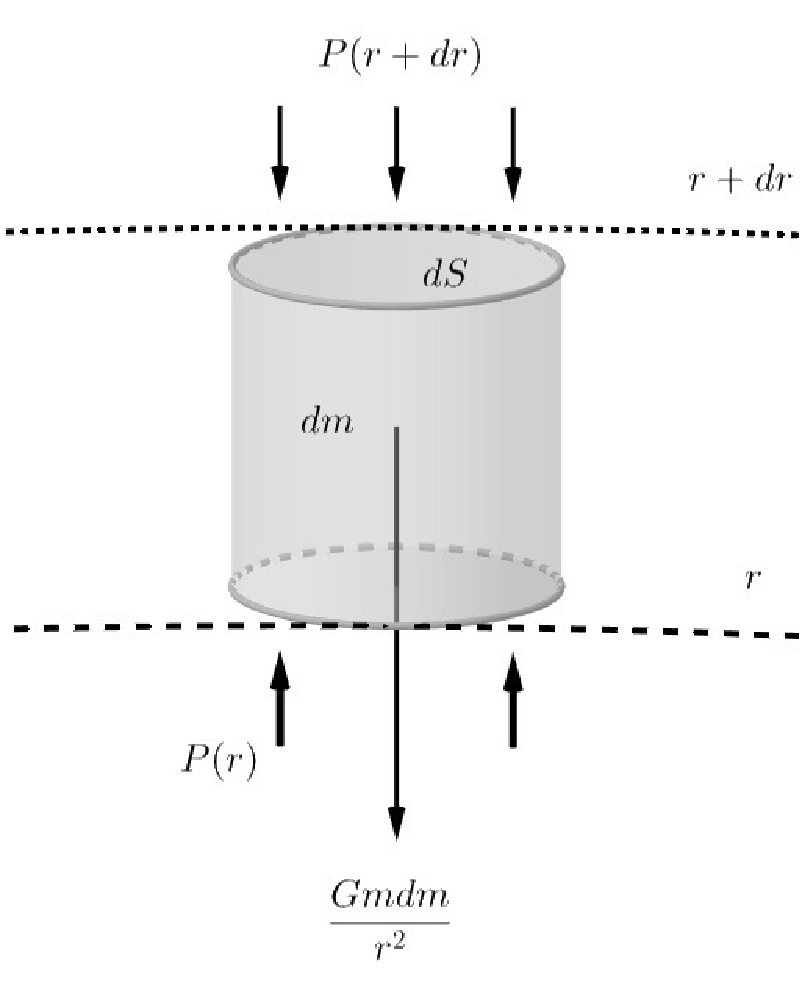
\includegraphics[scale=0.5]{images/cylindre}
	\caption[Cylindre de volume infinitésimal soumis à la force graviationnelle et à la pression radiative - figure réalisée avec GeoGebra]{Cylindre de volume infinitésimal soumis à la force graviationnelle et à la pression radiative}
	\label{Fig. 7.1}
\end{figure}\bigskip

Graphe fonction de l'indice polytropqiue choisi

\section{Masse de Chandrasekhar}

\begin{equation}\left( \dfrac{GM}{M_{n}}\right)^{n-1} \left( \dfrac{R}{R_{n}}\right)^{3-n}=\dfrac{\left[ \left( n+1\right)K\right]^n}{4\pi G}\end{equation}

\begin{equation}M_{n}=-\xi_{1}^{2}\left( \dfrac{d\theta}{d\xi}\right)_{\xi_{1}}\end{equation}

\begin{equation}R_{n}=\xi_{1}\end{equation}

\begin{equation}M=4\pi M_{3}\left(\dfrac{K}{\pi G}\right)^{3/2}\end{equation}

\begin{equation}R\propto M^{-\frac{1}{3}}\end{equation}

\begin{equation}\bar{\rho}\propto M R^{-3}\propto M^{2}\end{equation}

\begin{equation}k_{2}=\dfrac{hc}{8}\left(\dfrac{3}{\pi}\right)^{1/3} \dfrac{1}{m_{H}^{4/3}}\hspace{5pt}\mu_e^{-4/3}\end{equation}

\begin{equation}M_{Ch}=\dfrac{M_{3}\sqrt{1.5}}{4\pi}\left( \dfrac{hc}{Gm_{H}^{4/3}}\right)^{3/2}\hspace{5pt}\mu_{e}^{-2}\end{equation}

\begin{equation}M_{Ch}=5.83\hspace{3pt}\mu_{e}^{-2}M_\odot\end{equation}

\begin{equation}M_{Ch}=1.46\hspace{3pt}M_\odot\end{equation}